% TODO: add definiton of DC value, stuff from tutorials
\documentclass[landscape,a4paper]{extarticle}
\usepackage{relsize}
\usepackage{caption}
\usepackage{multicol}
\usepackage[top=2em,bottom=2em,left=2em,right=2em]{geometry}
\usepackage[framemethod=tikz]{mdframed}
\usepackage{microtype}
\usepackage{pdfpages}
\usepackage{amsmath, amssymb, amsthm}
\usepackage{anyfontsize}
\usepackage[shortlabels]{enumitem}
\usepackage{graphicx, float}
\usepackage{ulem}
\usepackage{xcolor}

\let\bar\overline
\setlength{\columnsep}{0.7em}

% Configure image directory
\graphicspath{{images/}}

\newenvironment{Figure}
  {\par\medskip\noindent\minipage{\linewidth}}
  {\endminipage\par\medskip}

% Remove caption labels
\captionsetup{labelformat=empty,labelsep=none}

% No paragraph indent
\setlength{\parindent}{0pt}

% No spaces between list items
\setlist[enumerate]{nosep, leftmargin=*}
\setlist[itemize]{nosep, leftmargin=*}

\newcommand{\sgn}{\text{sgn}}

% No spaces before and after math mode
\expandafter\def\expandafter\normalsize\expandafter{%
    \normalsize%
    \setlength\abovedisplayskip{0pt}%
    \setlength\belowdisplayskip{0pt}%
    \setlength\abovedisplayshortskip{-8pt}%
    \setlength\belowdisplayshortskip{2pt}%
}

\begin{document}
\fontsize{7}{9}\selectfont
\begin{multicols*}{5}
    \textbf{Euler's formula}
    \begin{align*}
        e^{j\theta}=\cos(\theta) + j\sin(\theta)\\
        e^{-j\theta}=\cos(\theta)-j\sin(\theta)
    \end{align*}

    \textbf{\uline{Chapter 1}}

    \textbf{1.2.2 Bounded signals}

    A continuous-time signal $x(t)$ is bounded if there exists an $M$ such that $0 < M < \infty$ and $\forall t \ |x(t)| \leq M$ (has an upper and lower range limit)

    \textbf{1.2.3 Absolutely integrable signals}

    A continuous-time signal $x(t)$ is absolutely integrable if 
    \[
        \int_{-\infty}^{\infty}|x(t)| dt < \infty
    \]

    \textbf{1.2.4 Periodc and aperiodic signals}

    Periodic: there is a non-zero positive value, $T$, satisfying 
    \[
        x(t)=x(t+T) \ \forall t \tag{1.1}
    \]

    Aperiodic: not periodic

    \textbf{1.2.6 Energy and Power Signals}

    \textbf{Energy signals}
    \[
        E = \int_{-\infty}^{\infty}|x(t)|^2 dt \tag{1.3a}
    \]
    
    \[
        x(t) \text{ is an energy signal} \iff 0 < E < \infty \tag{1.3b}
    \]
    \textbf{Power signals}
    \[
        P = \lim_{\tau \to \infty}\frac{1}{2\tau}\int_{-\tau}^{\tau}|x(t)|^2dt \tag{1.4a}
    \]

    \[
        x(t) \text{ is a power signal} \iff 0 < P < \infty \tag{1.4b}
    \]
    If $x(t)$ is a periodic signal, average power may be computed by
    \[
        \frac{1}{T}\int_0^T|x(t)|^2 dt
    \]
    \begin{itemize}
        \item Energy signals have 0 average power, bc E = finite implies P = 0
        \item Power signals have infinite total energy, bc P = finite implies $E = \infty$
        \item All bounded periodic signals are power signals
    \end{itemize}
    \textbf{u(t):}
    \begin{Figure}
        \centering
        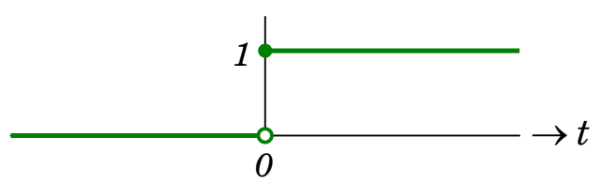
\includegraphics[width=0.8\linewidth]{images/unitStep.png}
    \end{Figure}
    \textbf{sgn(t):}
    \begin{Figure}
        \centering
        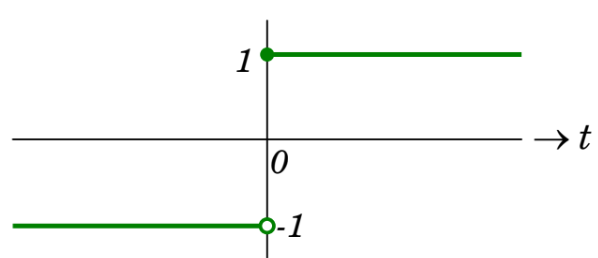
\includegraphics[width=0.8\linewidth]{images/signum.png}
    \end{Figure}
    \textbf{rect$\left( \frac{t}{T}\right)$:}
    \begin{Figure}
        \centering
        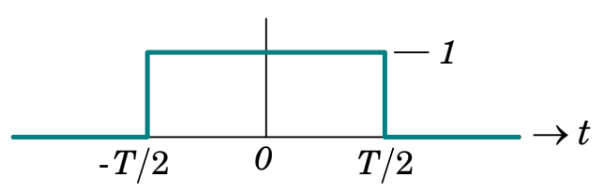
\includegraphics[width=0.8\linewidth]{images/rect.png}
    \end{Figure}
    \textbf{tri$\left( \frac{t}{T}\right)$:}
    \begin{Figure}
        \centering
        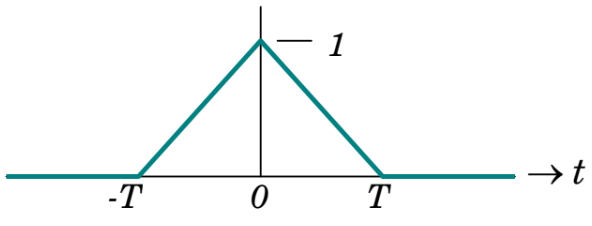
\includegraphics[width=0.8\linewidth]{images/tri.png}
    \end{Figure}
    \textbf{sinc$\left(\frac{t}{T}\right)$:}
    \begin{Figure}
        \centering
        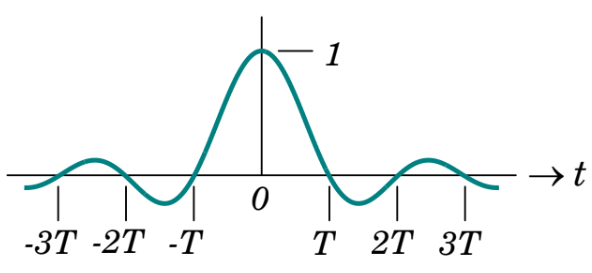
\includegraphics[width=0.8\linewidth]{images/sinc.png}
    \end{Figure}
    \textbf{$e^{-\alpha t}u(t)$: }
    \begin{Figure}
        \centering
        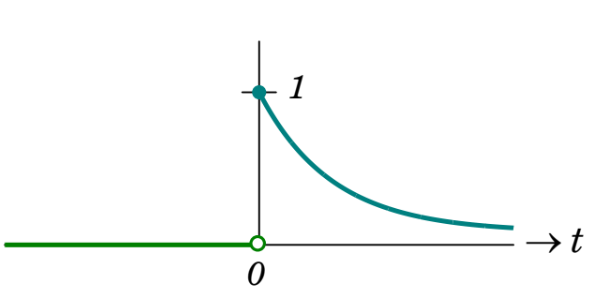
\includegraphics[width=0.8\linewidth]{images/rightSidedDecayingExp.png}
    \end{Figure}
    \textbf{$e^{-\alpha |t|}$: }
    \begin{Figure}
        \centering
        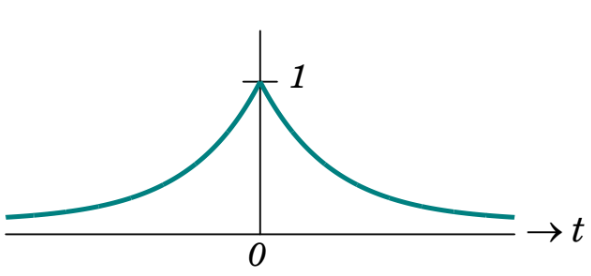
\includegraphics[width=0.8\linewidth]{images/twoSidedDecayingExp.png}
    \end{Figure}
    \textbf{Sinusoidal signals}
    \begin{align*}
        x(t)&=\mu \cos(\omega_0t+\phi)\\
        &= \mu\cos(2\pi f_0t + \phi)\\
        &= \mu\cos(\frac{2\pi t}{T} + \phi)
    \end{align*} \newline
    \[
        T_0=\frac{2\pi}{\omega_0}=\frac{1}{f_0}
    \]

    \textbf{\uline{Chapter 2}}

    \textbf{2.1 Time-domain Operations}

    \textbf{2.1.1 Time-Scaling}

    $x(\alpha t)$: Scale x-axis by a factor of $\frac{1}{\alpha}$

    $x(-t)$: Reflect about x-axis

    \textbf{2.1.2 Time-Shifting}

    $x(t-\beta)$:

    $\beta > 0$: Delaying $x(t)$ by $\beta$ units of time (translate right along x-axis)

    $\beta > 0$: Advancing $x(t)$ by $\beta$ units of time (translate left along x-axis)

    \textbf{2.1.5 Convolution of 2 Signals}

    $x(t)*y(t)=\int_{-\infty}^{\infty}x(\alpha)y(t-\alpha)\ d\alpha$

    \textbf{Properties of convolutions}
    \begin{enumerate}
        \item Commutative: $f * g = g * f$
        \item Associative: $f * (g * h) = (f * g) * h$
        \item Distributive: $f * (g + h) = (f * g) + (f * h)$
    \end{enumerate}

    \textbf{2.2 Dirac-$\delta$ function}

    \[
        \delta(t)=
        \begin{cases}
            \infty; &t=0\\
            0; &t\neq0
        \end{cases}
    \]
    \textbf{Properties: }
    \begin{enumerate}
        \item Symmetry:
        \[
            \delta(t)=\delta(-t) \tag{2.3}
        \]
        \item Sampling: 
        \[
            x(t)\delta(t-\lambda)=x(\lambda)\delta(t-\lambda) \tag{2.4}
        \]
        \item Sifting
        \begin{align*}
            &\int_{-\infty}^{\infty} x(t)\delta(t-\lambda)dt\\
            =\ &x(\lambda)\int_{-\infty}^{\infty}\delta(t-\lambda)dt=x(\lambda) \tag{2.5}
        \end{align*}
        \item Replication
        \begin{align*}
            &x(t)*\delta(t-\lambda)\\
            =&\int_{-\infty}^{\infty}x(\zeta)\delta(t-\zeta-\lambda)d\zeta\\
            =&\int_{-\infty}^{\infty}x(\zeta)\delta(\zeta-(t-\lambda))d\zeta=x(t-\lambda) \tag{2.6}
        \end{align*}
    \end{enumerate}
    \textbf{2.2.1 Dirac-$\delta$ Comb function}
    \begin{align*}
        &\sum_{n=-\infty}^{\infty}\delta(t-nT)\\
        &= \ldots+\delta(t+T)+\delta(t)+\delta(t-T) + \ldots
    \end{align*}

    \textbf{Convolution with Dirac-$\delta$ Comb function}
    \begin{align*}
        x_p(t)&=x(t)*\sum_n\delta(t-nT)\\
        &=\sum_n x(t-nT)
    \end{align*}
    $x(t)$ is known as the generating function.

    \textbf{Multiplication with the Dirac-$\delta$ Comb function}

    Used for sampling
    \begin{align*}
        x_s(t)&=x(t)\times\sum_n\delta(t-nT)\\
        &=\sum_nx(t)\times\delta(t-nT)\\
        &=\sum_nx(nT)\delta(t-nT)
    \end{align*}
    
    \textbf{\uline{Chapter 3}}

    \textbf{3.2 Spectrum of a Sinusoid}

    \textbf{Spectrum of a Complex Exponential Signal}
    \[
        \tilde{x}(t)=\mu e^{j(2\pi f_0t+\phi)} = \mu e^{j\phi} \times e^{j2\pi f_0t},
    \]where $\mu$: magnitude spectrum, $\phi$: phase spectrum, $f_0$: frequency

    \textbf{Spectrum of a Cosine Signal}
    \begin{align*}
        &\mu \cos(2\pi f_0t + \phi)\\
        % = \ &\frac{\mu}{2}e^{j\phi}e^{j2\pi f_0t} + \frac{\mu}{2} \mu e^{-j\phi}e^{-j2\pi f_0t}\\
        = \ &\frac{\mu}{2}e^{j\phi}e^{j2\pi f_0t} + \frac{\mu}{2}  e^{j(-\phi)}e^{j2\pi (-f_0)t}
    \end{align*}\\
    \textbf{Spectrum of a Sine Signal}
    \begin{align*}
        \mu\sin(2\pi f_0 t + \phi)
        % =\ &\frac{\mu}{2}e^{j(\phi - 0.5\pi)}e^{j2\pi f_0t} + \frac{\mu}{2}e^{-j(\phi-0.5\pi)}e^{j2\pi (-f_0)t}\\
        =\ &\frac{\mu}{2}e^{j(\phi - 0.5\pi)}e^{j2\pi f_0t} \\
        + \ &\frac{\mu}{2}e^{j(-\phi+0.5\pi)}e^{j2\pi (-f_0)t}
    \end{align*}
    \textbf{Complex exponential Fourier Series}
    \begin{align*}
        x_p(t)&=\sum_{k=-\infty}^{\infty}c_ke^{j2\pi kt/T_p}\\
        &=\sum_{k=-\infty}^{\infty}c_ke^{j2\pi kf_pt} \tag{3.1a}
    \end{align*}
    \begin{align*}
        c_k=\frac{1}{T_p}\int_{t_0}^{t_0+T_p}x_p(t)e^{-j2\pi kt/T_p}dt, k \in \mathbb{Z} \tag{3.1b}
    \end{align*}

    \textbf{Trigonometric Fourier Series}
    \begin{align*}
        x_p(t) = \ a_0 + 2\sum_{k=1}^{\infty} [ &a_k \cos(2\pi kt/T_p) \\
        &+ b_k \sin(2\pi kt/T_p)]
    \end{align*}
    \begin{align*}
        a_k&=\frac{1}{T_p}\int_{t_0}^{t_0+T_p}x_p(t)\cos(2\pi kt/T_p)dt; k \geq 0\\
        b_k&=\frac{1}{T_p}\int_{t_0}^{t_0+T_p}x_p(t)\sin(2\pi kt/T_p)dt; k > 0
        \tag{3.2}
    \end{align*}

    \textbf{\uline{Chapter 4}}\\
    \textbf{Dirichlet Conditions}\\
    Conditions for existence of Fourier Transform:
    \begin{enumerate}
        \item $x(t)$ has only a finite number of maxima and minima in any finite time interval
        \item $x(t)$ has only a finite number of discontinuities in any finite time interval
        \item $x(t)$ is absolutely integrable
    \end{enumerate}
    3 is weak Dirichlet condition: satisfied by most energy signals, violated by all power signals.\\
    \textbf{4.1 Fourier Transform}\\
    \textbf{Forward Fourier Transform}
    \[
        X(f)=\int_{-\infty}^{\infty}x(t)e^{-j2\pi ft}dt \tag{4.1a}
    \]
    \textbf{Inverse Fourier Transform}
    \[
       x(t)=\int_{-\infty}^{\infty}X(f)e^{j2\pi ft}df \tag{4.1b} 
    \]

    \textbf{Spectrum of exponentially decaying pulse}
    \begin{align*}
        x(t) &= Ae^{-\alpha t} u(t)\\
        & = \begin{cases}
            Ae^{-\alpha t}; &t > 0\\
            0; &t < 0
        \end{cases}\\
        &\text{Assume } \alpha > 0
    \end{align*}

    \[
        X(f) = \frac{A}{\alpha + j 2\pi f}
    \]

    \textbf{4.2 Properties of Fourier Transform}
    \begin{itemize}
        \item $X(f)=\Im\{x(t)\}$ denotes the Fourier transform of $x(t)$
        \item $x(t)={\Im}^{-1}\{X(f)\}$ denotes the inverse Fourier transform of $X(f)$
        \item $x(t) \rightleftarrows X(f)$ denotes a Fourier transform pair with the time-domain on the LHS and frequency-domain on the RHS.
    \end{itemize}
    \textbf{Linearity}

    If $x_1(t) \rightleftarrows X_1(f)$ and $x_2(t) \rightleftarrows X_2(f)$, then \[
        \alpha x_1(t) + \beta x_2(t)\rightleftarrows \alpha X_1(f) + \beta X_2 (f) \tag{4.2}
    \]

    \textbf{Time Scaling}

    \[
        x(\beta t) \rightleftarrows \frac{1}{|\beta|} X\left( \frac{f}{\beta}\right) \tag{4.3}
    \]

    \textbf{Duality}

    \[
        X(t) \rightleftarrows x(-f) \tag{4.4}
    \]

    \centerline{or}

    \[
        X(-t) \rightleftarrows x(f)
    \]

    \textbf{Time Shifting}

    \[
        x(t-t_0) \rightleftarrows X(f)e^{-j2\pi ft_0} \tag{4.5}
    \]

    \[
        x(t+t_0) \rightleftarrows X(f)e^{j 2 \pi f t_0}
    \]

    \textbf{Frequency Shifting (Modulation)}

    \[
        x(t)e^{j2\pi f_0t} \rightleftarrows X(f-f_0) \tag{4.6}
    \]

    \[
        x(t)e^{-j2\pi f_0t} \rightleftarrows X(f+f_0)
    \]

    \textbf{Differentiation in the Time Domain}

    \[
        \frac{d}{dt}x(t) \rightleftarrows j2\pi f \cdot X(f) \tag{4.7}
    \]

    \textbf{Integration in the Time Domain}

    \[
        \int_{-\infty}^{t}x(\tau)\ d\tau \rightleftarrows \frac{1}{j2\pi f}X(f) + \frac{1}{2}X(0)\delta(f) \tag{4.8}
    \]

    \textbf{Convolution in the Time Domain / Multiplication in the Frequency Domain}
    \begin{align*}
        &x_1(t) * x_2(t) \\
        = &\int_{-\infty}^{\infty}x_1(\alpha)x_2(t-\alpha)\ d\alpha \rightleftarrows X_1(f)X_2(f) \tag{4.9a}
    \end{align*}

    \textbf{Multiplication in the Time Domain / Convolution in the Frequency Domain} 
    \begin{align*}
        x_1(t)x_2(t) \rightleftarrows &\int_{-\infty}^{\infty} X_1(\alpha)X_2(f-\alpha)\ d\alpha \\=&X_1(f)*X_2(f) \tag{4.9b}
    \end{align*}

    \textbf{4.3 Spectral properties of a REAL signal}
    \begin{itemize}
        \item If $x(t)$ is \textbf{REAL} ($x^*(t)=x(t)$), then
        \begin{itemize}
            \item $X(f)$ is conjugate symmetric \textcolor{black!70}{($X^*(f)=X(f)$)}
            \item $|X(f)|$ is even \textcolor{black!70}{($|X(f)|=|X(-f)|$)}
            \item $\angle X(f)$ is odd \textcolor{black!70}{($\angle X(f)=-\angle X(-f)$)}
        \end{itemize}
        \item If $x(t)$ is \textbf{REAL} and \textbf{EVEN} ($x^*(t)=x(t) \wedge x(-t)=x(t)$), then
        \begin{itemize}
            \item $X(f)$ is real \textcolor{black!70}{($X^*f=X(f)$)}
            \item $X(f)$ is even \textcolor{black!70}{($X(-f)=X(f)$)}
        \end{itemize}
        \item If $x(t)$ is \textbf{REAL} and \textbf{ODD} ($x^*(t)=x(t) \wedge x(-t)=-x(t)$), then
        \begin{itemize}
            \item $X(f)$ is imaginary \textcolor{black!70}{($X^*(f) = -X(f)$)}
            \item $X(f)$ is odd \textcolor{black!70}{($X(-f)=-X(f)$)}
        \end{itemize}
    \end{itemize}

    The above can apply to Fourier series coefficients of periodic signals too:
    \begin{itemize}
        \item $x_p(t)$ is \textbf{REAL}
        \begin{itemize}
            \item $c_k$ is conjugate symmetric \textcolor{black!70}{($c_k^* = c_{-k}$)}
            \item $|c_k|$ has even symmetry \textcolor{black!70}{($|c_k|=|c_{-k}|$)}
            \item $\angle c_k$ has odd symmetry \textcolor{black!70}{($\angle c_k = -\angle c_{-k}$)}
        \end{itemize}
        \item $x_p(t)$ is \textbf{REAL} and \textbf{EVEN}
        \begin{itemize}
            \item $c_k$ is real \textcolor{black!70}{($c_k^*=c_k$)}
            \item $c_k$ is even \textcolor{black!70}{($c_k=c_{-k}$)}
        \end{itemize}
        \item $x_p(t)$ is \textbf{REAL} and \textbf{ODD}
        \begin{itemize}
            \item $c_k$ is imaginary \textcolor{black!70}{($c_k^*=-c_k$)}
            \item $c_k$ is odd \textcolor{black!70}{($c_k=-c_{-k}$)}
        \end{itemize}
    \end{itemize}
    \textbf{4.4 Spectrum of Signals that are not Absolutely Integrable}

    \[
        \Im\{K\delta (t)\} = \int_{-\infty}^{\infty}K \delta(t)e^{-j2\pi  ft}dt=K \tag{4.13}
    \]

    By duality, $\Im\{K\}=K\delta(f)$
    \begin{Figure}
        \centering
        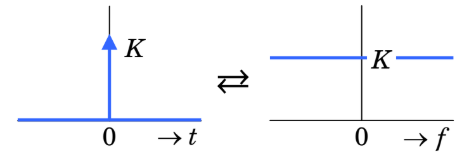
\includegraphics[width=0.8\linewidth]{images/fourierOfImpulse.png}
    \end{Figure}
    \begin{Figure}
        \centering
        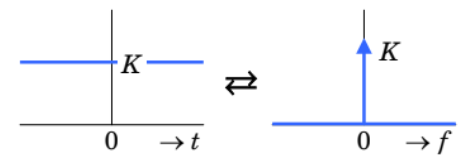
\includegraphics[width=0.8\linewidth]{images/fourierOfConstant.png}
    \end{Figure}

    \textbf{4.4.1 Spectrm of Unit Step and Signum function}

    \[
        \Im\{u(t)\}=\frac{1}{j2\pi f} + \frac{1}{2}\delta(f)
    \]

    \[
        \Im\{\text{Sgn}(t)\} = \frac{1}{j\pi f}
    \]

    \textbf{4.4.2 Continuous-Frequency Spectrum of Periodic Signals}

    The following make use of the fact that
    \[
        \Im\{k\}=K\delta(f) \tag{4.14}
    \]
    \textbf{DC}
    \begin{align*}
        &x_{dc}(t)=K \\
        &X_{dc}(f)=\Im\{k\}=K\Im\{1\}=K\delta(f)
    \end{align*}
    \begin{Figure}
        \centering
        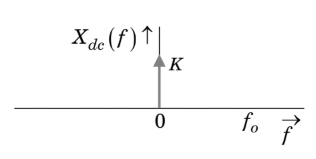
\includegraphics[width=0.8\linewidth]{images/continuousSpectrum_DC.png}
    \end{Figure}    
    \textbf{Complex Exponential}
    \begin{align*}
        &\tilde{x}(t) = Ke^{j2\pi f_0t} \\
        &\tilde{X}(f)=\Im\{Ke^{j2\pi f_0t}\} = K\delta(f-f_0)
    \end{align*}
    \begin{Figure}
        \centering
        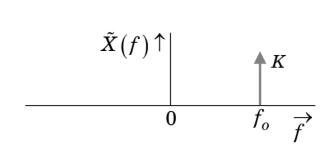
\includegraphics[width=0.8\linewidth]{images/continuousSpectrum_complexExponential.png}
    \end{Figure}
    \textbf{Cosine}
    \begin{align*}
        &\Im\{K\cos{(2\pi f_0t)}\}\\
        =&\frac{K}{2}\delta(f-f_0)+\frac{K}{2}\delta(f+f_0)
    \end{align*}
    \begin{Figure}
        \centering
        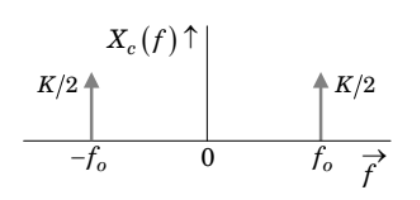
\includegraphics[width=0.8\linewidth]{images/continuousFreqSpectrum_Cos.png}
    \end{Figure}
    \textbf{Sine}
    \begin{align*}
        &\Im\{K\sin(2\pi f_0 t)\}\\
        = &\frac{K}{j2}\delta(f-f_0) - \frac{K}{j2}\delta(f+f_0)
    \end{align*}

    \[
    \text{where } \begin{cases}
            |X_s(f)|&=\frac{K}{2}\delta(f-f_0)\\
            &\quad+ \ \frac{K}{2}\delta(f+f_0)\\\\
            \angle X_s(f)&= \begin{cases}
                -\pi/2, &\quad f=f_0\\
                \pi/2, &\quad f=-f_0
            \end{cases}
        \end{cases}
    \]

    \begin{Figure}
        \centering
        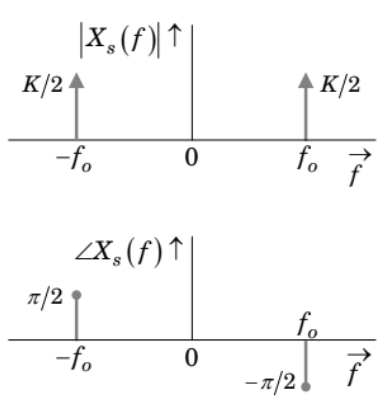
\includegraphics[width=0.8\linewidth]{images/continuousFreqSpectrum_Sine.png}
    \end{Figure}

    \textbf{Arbitrary periodic signals}

    Let $x_p(t)$ be a periodic signal with period $T_p$ and fundamental frequency $f_p$
    \[
        X_p(f)=\sum_{k=-\infty}^{\infty}c_k\delta (f-kf_p) \tag{4.16} 
    \]
    \begin{Figure}
        \centering
        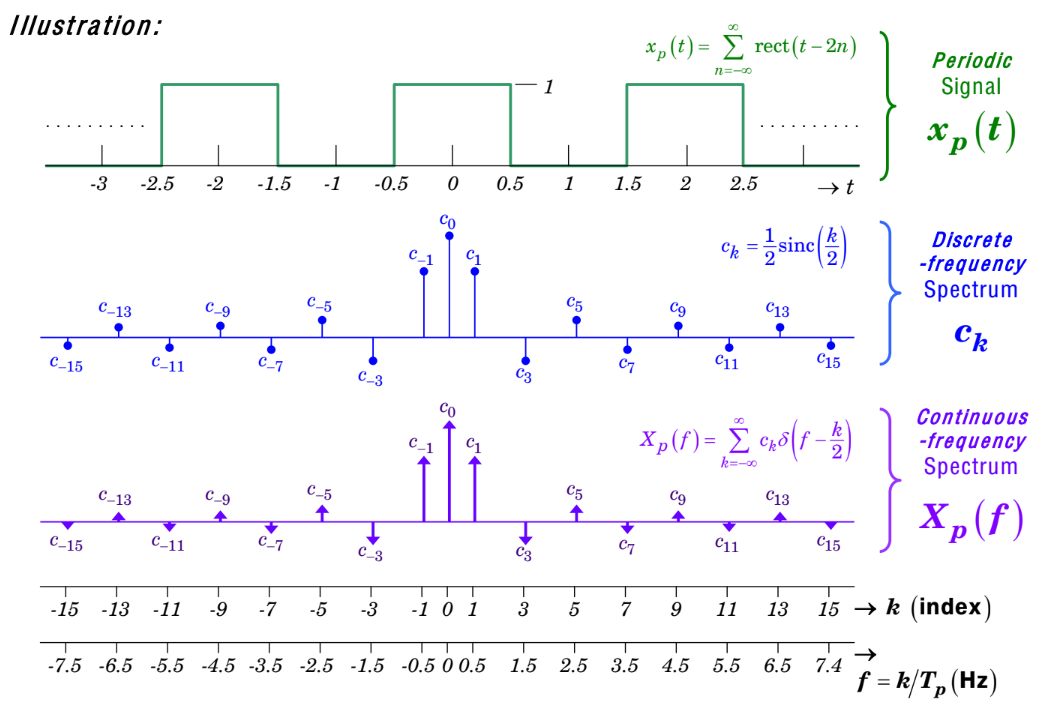
\includegraphics[width=\linewidth]{images/continuousFreqSpectrum_periodic.png}
    \end{Figure}

    \textbf{4.4.2.1 Spectrum of Dirac-$\delta$ Comb function}

    \[
        \text{comb}_\lambda(t) \triangleq \sum_n\delta(t-n\lambda)
    \]

    \begin{Figure}
        \centering
        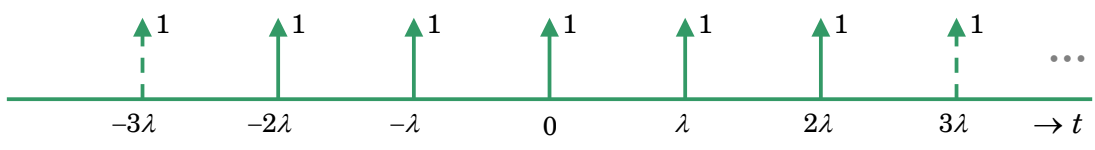
\includegraphics[width=\linewidth]{images/comb.png}
    \end{Figure}

    \[
        c_k=\frac{1}{\lambda}
    \]
    \begin{Figure}
        \centering
        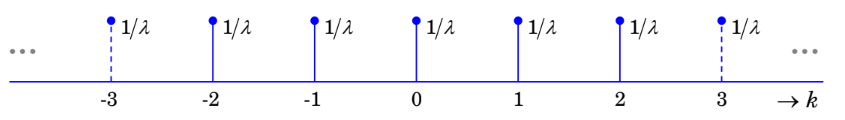
\includegraphics[width=\linewidth]{images/discreteFreqSpec_comb.png}
    \end{Figure}
    \begin{align*}
        \Im\{\text{comb}_\lambda(t)\} &= \text{COMB}_\lambda(f)\\
        &=\frac{1}{\lambda}\sum_k\delta(f-k/\lambda)
    \end{align*}
    \begin{Figure}
        \centering
        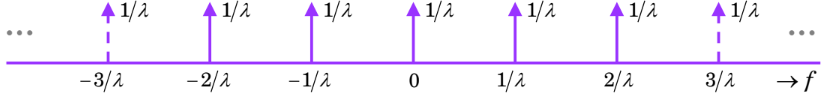
\includegraphics[width=\linewidth]{images/continuousFreqSpectrum_comb.png}
    \end{Figure}
    
    \textbf{\uline{Chapter 5}}

    \textbf{5.1 Energy Spectral Density (ESD)}

    Total energy of a signal $x(t)$ is defined as 
    \[
        E=\int_{-\infty}^{\infty}|x(t)|^2 dt \text{ (Joules)} \tag{5.1}
    \]
    \textbf{Rayleigh Energy Theorem}
    \[
        E=\int_{-\infty}^{\infty}|x(t)|^2dt=\int_{-\infty}^{\infty}|X(f)|^2df \tag{5.2},
    \]
    where $X(f)=\Im\{x(t)\}$ is the spectrum of the signal.

    \textbf{Energy Spectral Density}
    \[
        E_x(f)=|X(f)|^2 \text{ Joules Hz}^{-1}\tag{5.3}
    \]
    \textbf{Properties of $E_x(f)$}
    \begin{enumerate}
        \item $E_x(f)$ is a real function of $f$
        \item $E_x(f) \geq 0 \quad\forall f$
        \item $E_x(f)$ is an even function of $f$ if $x(t)$ is real.
    \end{enumerate}

    \textbf{5.2 Power Spectral Density (PSD)}

    In the time-domain, the average power of a signal $x(t)$ is defined as 
    \[
        P=\lim_{\tau \to \infty} \frac{1}{2\tau}\int_{-\tau}^{\tau}|x(t)|^2 dt \tag{5.4}
    \]
    Windowed version of $x(t)$:
    \[
        x_W(t)=x(t)\text{rect}\left(\frac{t}{2W}\right) \tag{5.5}
    \]
    \textbf{Parseval Power Theorem}
    \begin{align*}
        P&=\lim_{W \to \infty}\frac{1}{2W}\int_{-W}^{W}|x(t)|^2dt\\
        &=\int_{-\infty}^{\infty}\lim_{W \to \infty}\frac{1}{2W}|X_W(f)|^2df \tag{5.9}
    \end{align*}
    \textbf{Power Spectral Density}
    \[
        {P_x(f)=\lim_{W \to \infty}\frac{1}{2W}|X_W(f)|^2} \text{ Watts Hz}^{-1} \tag{5.10}
    \]
    \textbf{Properties of $P_x(f)$}
    \begin{enumerate}
        \item $P_x(f)$ is a real function of $f$
        \item $P_x(f) \geq 0 \quad \forall f$
        \item $P_x(f)$ is an even function of $f$ if $x(t)$ is real.
    \end{enumerate}

    \textbf{5.2.1 PSD of Periodic Signals}

    From chapter 4 equation 4.16:
    \[
        X_p(f)=\sum_{k=-\infty}^{\infty}c_k \delta (f-kf_p)
    \]
    \textbf{PSD of $x_p(t)$}
    \[
        P_x(f)=\sum_{k=-\infty}^{\infty}|c_k|^2\delta (f-kf_p) \tag{5.12}
    \]
    \textbf{Average power of $x_p(t)$}
    \[
        P=\int_{-\infty}^{\infty}P_x(f)df=\sum_{k=-\infty}^{\infty}|c_k|^2 \tag{5.13}
    \]
    \textbf{5.3 Bandwidth}

    \textbf{5.3.1 Bandlimited Signals}

    \textbf{Lowpass signal}

    A signal $x(t)$ is said to be a bandlimited lowpass signal if its magnitude spectrum is concentrated around 0 Hz, and at the same time satisfies
    \[
        |X(f)|=0; \quad |f| > B \tag{5.14}
    \]
    where B is defined as the bandwidth of the signal. 
    \begin{Figure}
        \centering
        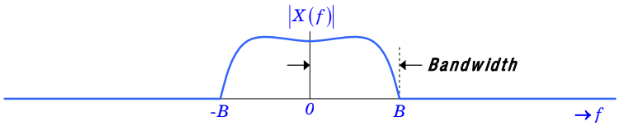
\includegraphics[width=\linewidth]{images/bandlimitedLowpassSignal.png}
    \end{Figure}
    \textbf{Bandpass signal}

    A signal $x(t)$ is said to be a bandlimited bandpass signal if its magnitude spectrum is concentrated around a non-zero center frequency $f_c$, and at the same time satisfies \[
        |X(f)|=0; \quad ||f|-f_c|>B/2 \tag{5.15}
    \]
    where B is defined as the bandwidth of the signal
    \begin{Figure}
        \centering
        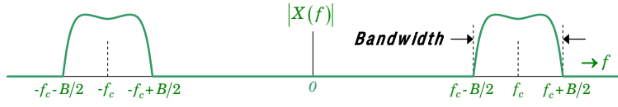
\includegraphics[width=\linewidth]{images/bandlimitedBandpassSignal.png}
    \end{Figure}
    \textbf{5.3.2 Signals with Unrestricted Band}

    \textbf{5.3.2.1 3dB Bandwidth}

    \textbf{Lowpass signal:}
    The frequency where $|X(f)|=|X(0)|/\sqrt{2}$ first occurs (or where $|X(f)|^2=|X(0)|^2/2$ first occurs) when $f$ is increased from 0 Hz.
    \begin{Figure}
        \centering
        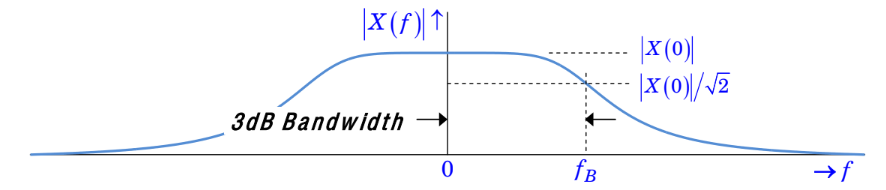
\includegraphics[width=\linewidth]{images/3dB_lowpass.png}
    \end{Figure}

    \textbf{Bandpass signal:}
    \begin{Figure}
        \centering
        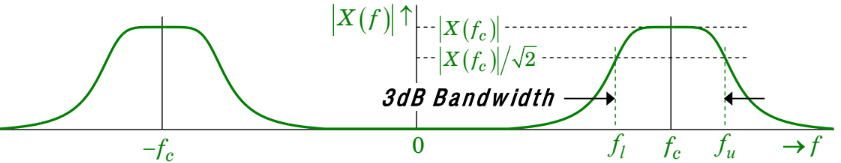
\includegraphics[width=\linewidth]{images/3dB_bandpass.png}
    \end{Figure}
    
    \textbf{5.3.2.2 1st-null Bandwidth}

    \textbf{Lowpass signal: } The frequency at which $|X(f)|=0$ first occurs when $f$ is increased from 0 Hz:
    \begin{Figure}
        \centering
        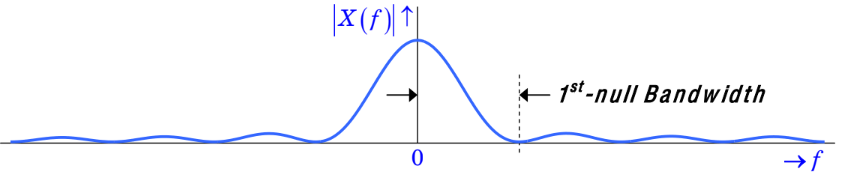
\includegraphics[width=\linewidth]{images/1stNull_lowpass.png}
    \end{Figure}
    \textbf{Bandpass signal: }
    \begin{Figure}
        \centering
        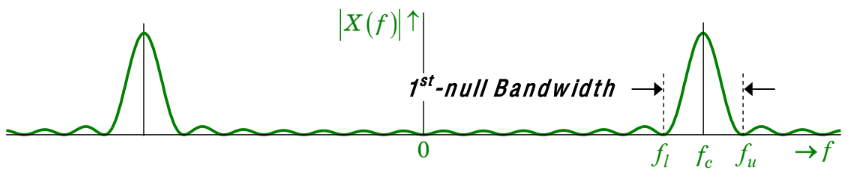
\includegraphics[width=\linewidth]{images/1stNull_bandpass.png}
    \end{Figure}

    \textbf{5.3.2.3 M\% Energy Containment Bandwidth}

    Smallest bandwidth that contains at least M\% of the total signal energy $E = \int_{-\infty}^{\infty}E_x(f)\ df$

    \textbf{Lowpass:}
    \begin{Figure}
        \centering
        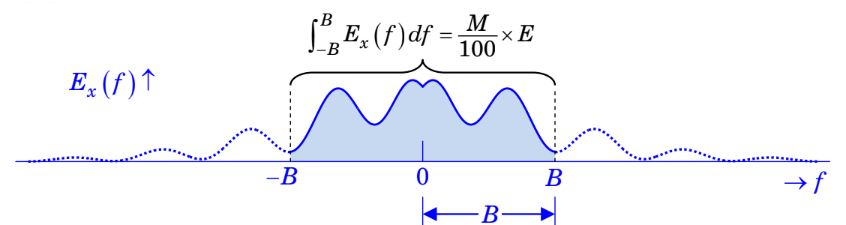
\includegraphics[width=\linewidth]{images/MPercentEnergy_lowpass.png}
    \end{Figure}
    \textbf{Bandpass:}
    \begin{Figure}
        \centering
        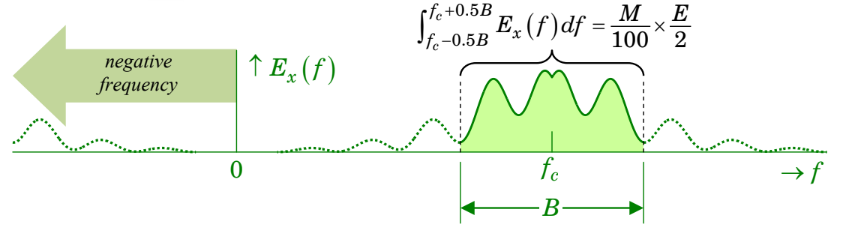
\includegraphics[width=\linewidth]{images/MPercentEnergy_bandpass.png}
    \end{Figure}

    \textbf{5.3.2.4 M\% Power Containment Bandwidth}

    The smallest bandwidth that contains at least M\% of the average signal power. For a periodic signal, the aerage power is given by
    \[
        P = \int_{-\infty}^{\infty}P_x(f)df=\sum_{k=-\infty}^{\infty}|c_k|^2
    \]
    where $f_p$(Hz) is the fundamental frequency and $c_k$'s are the Fourier series coefficients.
    \begin{Figure}
        \centering
        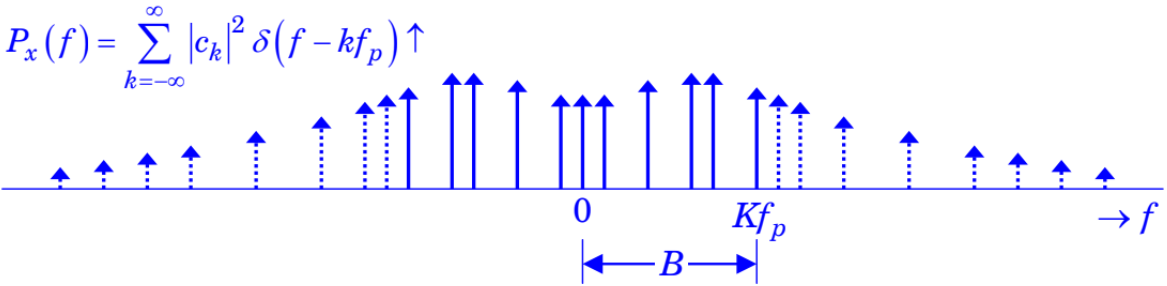
\includegraphics[width=\linewidth]{images/MPercentPower.png}
    \end{Figure}
    \[
        B = Kf_p
    \]
    where $K$ is the smallest positive integer that satisfies 
    \[
        \sum_{k=-k}^{K}|c_k|^2 \geq \frac{M}{100} \times P
    \]

    \textbf{Random stuff}
    
    \begin{align*}
        \angle j 2\pi f &= \tan^{-1}\left(\frac{2\pi f}{0}\right)\\
        &= \begin{cases}
            \tan^{-1}(\infty) &\text{if }f > 0\\
            \tan^{-1}(-\infty) &\text{if }f < 0
        \end{cases}\\
        &= \begin{cases}
            0.5 \pi &\text{if } f>0\\
            -0.5 \pi &\text{if } f < 0
        \end{cases}\\
        &= 0.5\pi \sgn(f)
    \end{align*}

\end{multicols*}
\end{document}
